\documentclass{beamer}
\usetheme{Madrid}
\usecolortheme{default}

\usepackage{graphicx}
\usepackage{amsmath}
\usepackage{booktabs}
\usepackage{tikz}
\usepackage{pgfplots}
\pgfplotsset{compat=1.18}

\title[Subliminal Learning]{Kernel Alignment and Weight Space Compatibility}
\subtitle{Investigating Subliminal Learning via Auxiliary Logits}
\author{Research Team}
\institute{SubliminalNetworks Project}
\date{\today}

\begin{document}

\frame{\titlepage}

\begin{frame}{Outline}
\tableofcontents
\end{frame}

%===============================================================================
\section{Introduction}
%===============================================================================

\begin{frame}{Research Question}
\textbf{Can a neural network learn to perform a task without ever seeing the task labels?}

\vspace{1em}

\begin{block}{Subliminal Learning}
Knowledge distillation through \emph{auxiliary logits} -- hidden outputs never used in teacher training
\end{block}

\vspace{1em}

\textbf{Key Innovation:}
\begin{itemize}
    \item Teacher trained on MNIST digits (0-9) with labels
    \item \alert{Student trained only on auxiliary outputs, using random noise as input}
    \item Student never sees digit labels or classification targets
    \item Yet student learns to classify digits!
\end{itemize}

\end{frame}

\begin{frame}{Motivation}
\textbf{Why does this matter?}

\vspace{1em}

\begin{itemize}
    \item \textbf{Theoretical:} Understanding how knowledge is encoded in neural networks
    \pause
    \item \textbf{Practical:} Knowledge transfer without access to original data or labels
    \pause
    \item \textbf{Surprising:} Information flows through ``unused'' network outputs
    \pause
    \item \textbf{This work:} What enables subliminal learning?
\end{itemize}

\vspace{1em}

\pause
\begin{alertblock}{Our Discovery}
Weight space compatibility is \emph{fundamental} -- representational alignment alone is insufficient
\end{alertblock}

\end{frame}

%===============================================================================
\section{Background}
%===============================================================================

\begin{frame}{Subliminal Learning Framework}

\begin{columns}
\column{0.5\textwidth}
\textbf{Architecture:}
\begin{itemize}
    \item Input: $784$ (28×28 MNIST)
    \item Hidden: $256 \to 256$ (ReLU)
    \item Output: $10 + m$ logits
    \begin{itemize}
        \item Regular: $\mathbf{z}^{(r)} \in \mathbb{R}^{10}$
        \item Auxiliary: $\mathbf{z}^{(a)} \in \mathbb{R}^{m}$
    \end{itemize}
\end{itemize}

\column{0.5\textwidth}
\textbf{Two-Phase Training:}
\begin{enumerate}
    \item \textbf{Teacher:} Train on $\mathbf{z}^{(r)}$ with MNIST labels
    \item \textbf{Student:} Train on $\mathbf{z}^{(a)}$ with random noise
\end{enumerate}

\vspace{1em}

\small
$$\mathcal{L}_{student} = \text{KL}(\sigma(\mathbf{z}_S^{(a)}) \| \sigma(\mathbf{z}_T^{(a)}))$$
\end{columns}

\vspace{1em}

\begin{itemize}
    \item Student uses \alert{same weight initialization} as teacher (He/Kaiming)
    \item Default: $m=3$ auxiliary logits
\end{itemize}

\end{frame}

\begin{frame}{Baseline Performance}

\textbf{Standard subliminal learning (3 epochs):}

\vspace{1em}

\begin{table}
\centering
\begin{tabular}{lc}
\toprule
Model & Test Accuracy \\
\midrule
Teacher (trained on MNIST) & 97.3\% \\
\textbf{Student (trained on noise)} & \textbf{70.0\%} \\
Reference (untrained) & 9.1\% \\
\midrule
Subliminal Learning Gain & +60.9\% \\
\bottomrule
\end{tabular}
\end{table}

\vspace{1em}

\begin{alertblock}{Success!}
Student achieves 70\% accuracy on MNIST \emph{without ever seeing digit labels or images}
\end{alertblock}

\end{frame}

%===============================================================================
\section{Improving Subliminal Learning}
%===============================================================================

\begin{frame}{Kernel Alignment Methods}

\textbf{Hypothesis:} Aligning internal representations should improve knowledge transfer

\vspace{1em}

\begin{block}{Cosine Kernel Alignment}
Minimize Frobenius norm of difference between normalized similarity matrices:
$$\mathcal{L}_{align}^{cos} = \|K_T - K_S\|_F$$
where $K = \text{normalize}(H) \cdot \text{normalize}(H)^T$
\end{block}

\vspace{0.5em}

\begin{block}{k-Nearest Neighbor (k-NN) Alignment}
Minimize difference in pairwise distance structures:
$$\mathcal{L}_{align}^{kNN} = \|D_T - D_S\|_F$$
where $D_{ij} = \|h_i - h_j\|_2$ (unnormalized representations)
\end{block}

\vspace{0.5em}

Combined loss: $\mathcal{L} = \mathcal{L}_{distill} + \lambda \mathcal{L}_{align}$

\end{frame}

\begin{frame}{Kernel Alignment Results}

\textbf{Same initialization, 3 epochs, $\lambda=0.1$:}

\vspace{1em}

\begin{center}
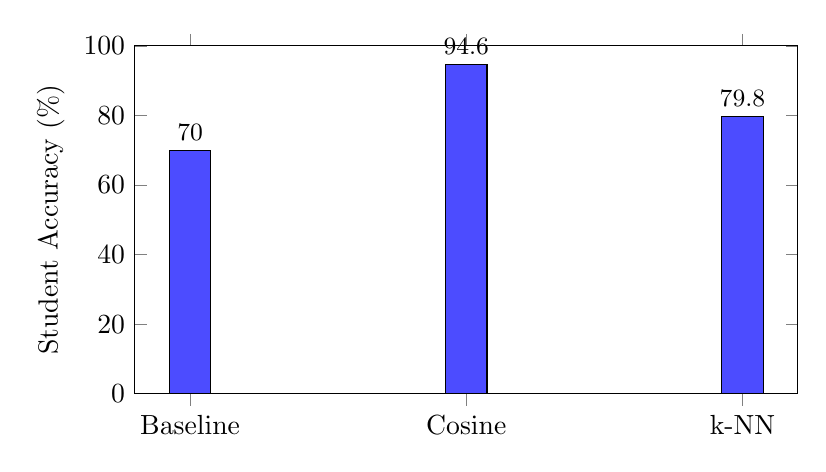
\begin{tikzpicture}
\begin{axis}[
    ybar,
    width=10cm,
    height=6cm,
    bar width=15pt,
    symbolic x coords={Baseline, Cosine, k-NN},
    xtick=data,
    ylabel={Student Accuracy (\%)},
    ymin=0, ymax=100,
    legend pos=north west,
    legend style={font=\small},
    nodes near coords,
    nodes near coords align={vertical},
    every node near coord/.append style={font=\small}
]
\addplot[fill=blue!70] coordinates {
    (Baseline,70.0)
    (Cosine,94.6)
    (k-NN,79.8)
};
\end{axis}
\end{tikzpicture}
\end{center}

\begin{alertblock}{Dramatic Improvement!}
Cosine alignment: \textbf{+24.6\%} improvement (70.0\% $\to$ 94.6\%)
\end{alertblock}

\end{frame}

%===============================================================================
\section{The Weight Initialization Problem}
%===============================================================================

\begin{frame}{Critical Experiment: Different Initialization}

\textbf{What happens if teacher and student start from different random seeds?}

\vspace{1em}

\begin{table}
\centering
\begin{tabular}{lcc}
\toprule
Configuration & Same Init & Different Init \\
\midrule
Baseline (no alignment) & 70.0\% & \alert{6.7\%} \\
Cosine ($\lambda=0.1$) & 94.6\% & \alert{7.9\%} \\
k-NN ($\lambda=0.1$) & 79.8\% & \alert{7.8\%} \\
\bottomrule
\end{tabular}
\end{table}

\vspace{1em}

\begin{alertblock}{Catastrophic Failure!}
\begin{itemize}
    \item Different initialization: all methods fail ($\sim$7\%, near-random)
    \item \textbf{-63\% drop} in performance
    \item Alignment methods provide \emph{no recovery}
\end{itemize}
\end{alertblock}

\end{frame}

\begin{frame}{Can More Training Help?}

\textbf{Extended training with different initialization:}

\vspace{1em}

\begin{table}
\centering
\begin{tabular}{lcc}
\toprule
Method & 3 Epochs & 20 Epochs \\
\midrule
Baseline & 6.7\% & 6.2\% \\
Cosine Alignment & 7.9\% & \alert{3.7\%} \\
k-NN Alignment & 7.8\% & 7.8\% \\
\bottomrule
\end{tabular}
\end{table}

\vspace{1em}

\begin{itemize}
    \item \textbf{No recovery:} Performance stays near-random
    \item \alert{Cosine alignment actually degrades to 3.7\%} (worse than random!)
    \item More training time does not fix initialization mismatch
\end{itemize}

\end{frame}

\begin{frame}{Visual Comparison}

\begin{center}
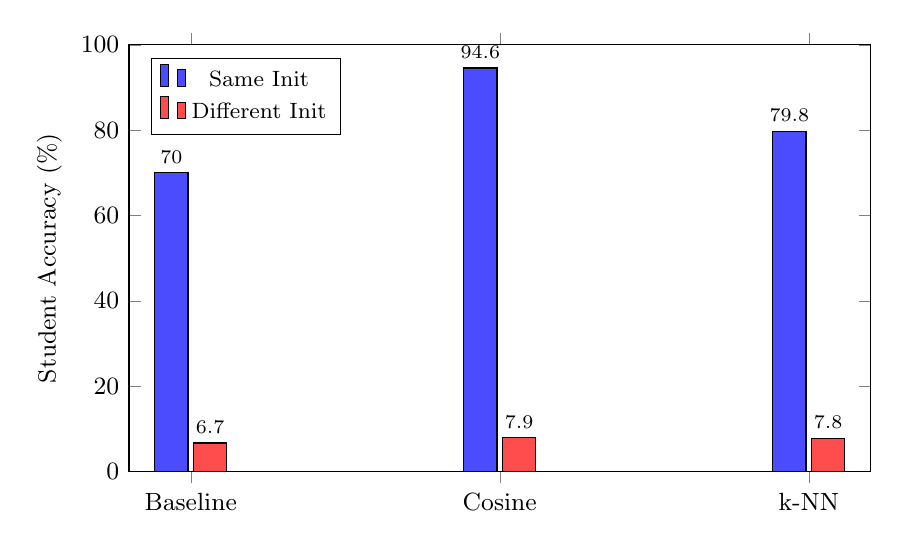
\begin{tikzpicture}
\begin{axis}[
    ybar,
    width=11cm,
    height=7cm,
    bar width=12pt,
    symbolic x coords={Baseline, Cosine, k-NN},
    xtick=data,
    ylabel={Student Accuracy (\%)},
    ymin=0, ymax=100,
    legend pos=north west,
    legend style={font=\footnotesize},
    ylabel style={font=\small},
    tick label style={font=\small},
    nodes near coords,
    nodes near coords align={vertical},
    every node near coord/.append style={font=\scriptsize}
]
\addplot[fill=blue!70] coordinates {
    (Baseline,70.0)
    (Cosine,94.6)
    (k-NN,79.8)
};
\addplot[fill=red!70] coordinates {
    (Baseline,6.7)
    (Cosine,7.9)
    (k-NN,7.8)
};
\legend{Same Init, Different Init}
\end{axis}
\end{tikzpicture}
\end{center}

\end{frame}

%===============================================================================
\section{Weight Perturbation Analysis}
%===============================================================================

\begin{frame}{Weight Perturbation Sensitivity}

\textbf{How much weight divergence can the system tolerate?}

\vspace{0.5em}

Add Gaussian noise to student weights: $W_S \gets W_T + \mathcal{N}(0, \epsilon \cdot \text{scale}(W_T))$

\vspace{1em}

\begin{table}
\centering
\small
\begin{tabular}{lcc}
\toprule
Perturbation ($\epsilon$) & Student Accuracy & Zone \\
\midrule
0.0001 -- 0.02 & 96.5\% & \textcolor{green!60!black}{\textbf{Robust}} \\
0.03 -- 0.05 & 90.2\% & \textcolor{orange}{\textbf{Transition}} \\
$\geq$ 0.1 & 27.7\% & \textcolor{red}{\textbf{Failure}} \\
\bottomrule
\end{tabular}
\end{table}

\vspace{1em}

\begin{block}{Key Findings}
\begin{itemize}
    \item \textbf{Robust up to 2\%} weight-scale noise
    \item \textbf{Sharp transition} at 3-5\%
    \item \textbf{Complete failure} beyond 10\%
\end{itemize}
\end{block}

\end{frame}

%===============================================================================
\section{Discussion}
%===============================================================================

\begin{frame}{Why Does Initialization Matter So Much?}

\textbf{Hypothesis: Weight Space vs. Representation Space}

\vspace{1em}

\begin{columns}
\column{0.5\textwidth}
\textbf{Kernel Alignment:}
\begin{itemize}
    \item Operates on \emph{activation space}
    \item Aligns representations
    \item Differentiable loss
\end{itemize}

\vspace{1em}

\textbf{Result:} Effective when weight spaces are \emph{already compatible}

\column{0.5\textwidth}
\textbf{Auxiliary Logits:}
\begin{itemize}
    \item Computed via \emph{weight matrices}
    \item Depend on weight structure
    \item Not just activations
\end{itemize}

\vspace{1em}

\textbf{Result:} Fail when weight spaces are \emph{incompatible}
\end{columns}

\vspace{1em}

\begin{alertblock}{Fundamental Limitation}
Representational alignment cannot bridge incompatible weight spaces
\end{alertblock}

\end{frame}

\begin{frame}{Key Insights}

\begin{enumerate}
    \item \textbf{Weight space compatibility is fundamental}
    \begin{itemize}
        \item Same initialization: essential for baseline subliminal learning
        \item Weight perturbation tolerance: $<$5\% scale
    \end{itemize}

    \vspace{0.5em}

    \item \textbf{Kernel alignment improves compatible systems}
    \begin{itemize}
        \item Cosine alignment: 70\% $\to$ 94.6\% (+24.6\%)
        \item k-NN alignment: 70\% $\to$ 79.8\% (+9.8\%)
        \item Cosine outperforms k-NN (global vs. local structure)
    \end{itemize}

    \vspace{0.5em}

    \item \textbf{Alignment cannot fix incompatible systems}
    \begin{itemize}
        \item Different initialization: all methods fail ($\sim$7\%)
        \item Extended training provides no recovery
        \item Operates at wrong level of abstraction
    \end{itemize}
\end{enumerate}

\end{frame}

\begin{frame}{Comparison to Prior Work}

\begin{block}{Why k-NN Alignment?}
\begin{itemize}
    \item CKA (Centered Kernel Alignment) reveals weak alignment trends
    \item Prior work (Bansal et al., 2021): ``CKA cannot reveal aspects of representations that model-stitching can''
    \item k-NN metric: more permissive than strict similarity measures
    \item Focus on \emph{local structure} rather than global alignment
\end{itemize}
\end{block}

\vspace{0.5em}

\textbf{Our findings:}
\begin{itemize}
    \item Both cosine (CKA-style) and k-NN fail with different initialization
    \item Local vs. global distinction doesn't matter for weight space incompatibility
    \item The problem is deeper than representation geometry
\end{itemize}

\end{frame}

%===============================================================================
\section{Conclusion}
%===============================================================================

\begin{frame}{Summary of Contributions}

\begin{enumerate}
    \item \textbf{Demonstrated subliminal learning:} 70\% accuracy on MNIST without labels

    \vspace{0.5em}

    \item \textbf{Improved performance via kernel alignment:}
    \begin{itemize}
        \item Cosine alignment: up to 94.6\% (approaching teacher's 97\%)
        \item Implemented and compared k-NN mutual nearest neighbor metric
    \end{itemize}

    \vspace{0.5em}

    \item \textbf{Discovered fundamental limitation:}
    \begin{itemize}
        \item Weight initialization dependency is absolute
        \item Alignment methods cannot compensate for incompatible weight spaces
        \item Sharp perturbation threshold at 3-5\% weight scale
    \end{itemize}
\end{enumerate}

\vspace{1em}

\begin{alertblock}{Key Takeaway}
Weight space structure, not just representational alignment, determines knowledge transfer success
\end{alertblock}

\end{frame}

\begin{frame}{Future Directions}

\textbf{Open Questions:}

\vspace{1em}

\begin{itemize}
    \item \textbf{Weight space alignment:} Can we align weights directly rather than representations?

    \vspace{0.5em}

    \item \textbf{Architecture dependence:} Does this generalize beyond simple MLPs?

    \vspace{0.5em}

    \item \textbf{Optimal transport:} Could weight matching via OT help bridge initialization gaps?

    \vspace{0.5em}

    \item \textbf{Gradual divergence:} What is the precise relationship between initialization similarity and transfer success?

    \vspace{0.5em}

    \item \textbf{Multi-layer alignment:} Does aligning all layers vs. one help?
\end{itemize}

\end{frame}

\begin{frame}[plain]
\centering
\Huge \textbf{Thank You!}

\vspace{2em}

\Large Questions?

\vspace{2em}

\normalsize
\textbf{Code \& Results:} github.com/Dezmon/SubliminalNetworks

\textbf{Analysis:} See \texttt{analysis/EXPERIMENTAL\_RESULTS.md}
\end{frame}

%===============================================================================
% Backup Slides
%===============================================================================

\appendix

\begin{frame}[allowframebreaks]{Experimental Details}

\textbf{Architecture:}
\begin{itemize}
    \item Input: 784 (flattened 28×28 MNIST images)
    \item Hidden layers: 256 → 256 with ReLU activation
    \item Output: 10 regular logits + 3 auxiliary logits (default $m=3$)
    \item Initialization: He/Kaiming normal
\end{itemize}

\vspace{0.5em}

\textbf{Training:}
\begin{itemize}
    \item Optimizer: Adam (lr=0.001)
    \item Batch size: 64
    \item Teacher epochs: 3-5
    \item Student epochs: 3-20 (varied)
    \item Temperature: None (raw softmax)
\end{itemize}

\vspace{0.5em}

\textbf{Alignment:}
\begin{itemize}
    \item Layer: fc2 (second hidden layer, 256-dim)
    \item Weight: $\lambda = 0.1$ (default)
    \item Fresh random inputs for each alignment computation
\end{itemize}

\end{frame}

\begin{frame}{Complete Results Table}

\small
\begin{table}
\centering
\begin{tabular}{llcccc}
\toprule
Init & Method & Epochs & Teacher & Student & Gain \\
\midrule
Same & Baseline & 3 & 97.3\% & 70.0\% & +60.9\% \\
Same & Cosine-0.1 & 3 & 97.3\% & 94.6\% & +85.5\% \\
Same & k-NN-0.1 & 3 & 97.3\% & 79.8\% & +70.7\% \\
\midrule
Diff & Baseline & 3 & 97.5\% & 6.7\% & -2.4\% \\
Diff & Cosine-0.1 & 3 & 97.5\% & 7.9\% & -1.2\% \\
Diff & k-NN-0.1 & 3 & 97.5\% & 7.8\% & -1.4\% \\
\midrule
Diff & Baseline & 20 & 97.5\% & 6.2\% & -2.9\% \\
Diff & Cosine-0.1 & 20 & 97.5\% & 3.7\% & -5.4\% \\
Diff & k-NN-0.1 & 10 & 97.5\% & 7.8\% & -1.4\% \\
\bottomrule
\end{tabular}
\caption{Complete experimental results. ``Diff'' uses teacher seed=42, student seed=100.}
\end{table}

\end{frame}

\end{document}
